\documentclass[a4paper,10pt]{article}
%-----------------------------------------------------------
\usepackage[top=0.75in, bottom=0.75in, left=0.55in, right=0.85in]{geometry}
\usepackage{graphicx}
\usepackage{url}
\usepackage{palatino}
\usepackage{tabularx}
\fontfamily{SansSerif}
\selectfont

\usepackage[T1]{fontenc}
\usepackage
%[ansinew]
[utf8]
{inputenc}

\usepackage{color}
\definecolor{mygrey}{gray}{0.75}
\textheight=9.75in
\raggedbottom

\setlength{\tabcolsep}{0in}
\newcommand{\isep}{-2 pt}
\newcommand{\lsep}{-0.5cm}
\newcommand{\psep}{-0.6cm}
\renewcommand{\labelitemii}{$\circ$}

\pagestyle{empty}
%-----------------------------------------------------------
%Custom commands
\newcommand{\resitem}[1]{\item #1 \vspace{-2pt}}
\newcommand{\resheading}[1]{{\small \colorbox{mygrey}{\begin{minipage}{0.975\textwidth}{\textbf{#1 \vphantom{p\^{E}}}}\end{minipage}}}}
\newcommand{\ressubheading}[3]{
\begin{tabular*}{6.62in}{l @{\extracolsep{\fill}} r}
	\textsc{{\textbf{#1}}} & \textsc{\textit{[#2]}} \\
\end{tabular*}\vspace{-8pt}}
%-----------------------------------------------------------

\begin{document}
\hspace{0.5cm}\\[-0.2cm]



\textbf{Yash Jivrajani} \\
\indent E -001 Gokul Samruddhi, Gokul Township, \\
\indent Opp. Muljibhai Mehta School,  \\
\indent Virar (W) (401303) MH IND

\indent Email-id : \textbf{yashjivrajani7799@gmail.com} \\
\indent Mobile No.: \textbf{7066705121} \\
\indent Alt Mob No.: \textbf{7977660130} \\
\hspace*{14cm} 
\smash{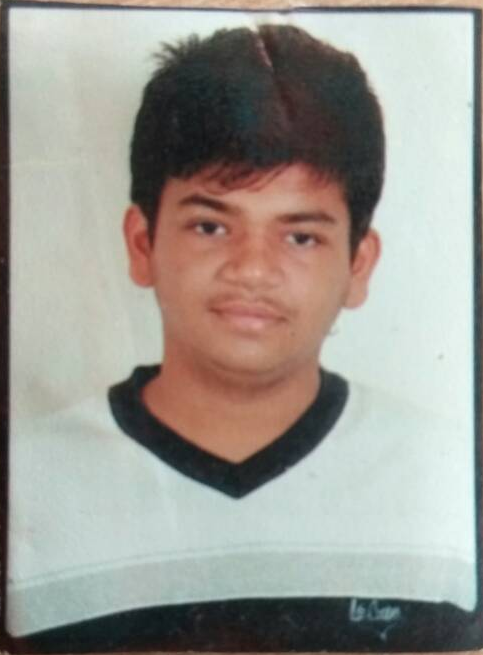
\includegraphics[width=3cm]{c}}

\indent{}
\resheading{\textbf{ACADEMIC DETAILS} }\\[\lsep]
\\ \\
\begin{table}[ht!]
\begin{center}
\indent \begin{tabular}{ l @{\hskip 0.1in} l @{\hskip 0.1in} l @{\hskip 0.1in} l @{\hskip 0.1in} l }
\hline
\textbf{Examination} & \textbf{University/Board} & \textbf{Institute} & \textbf{Year} & \textbf{CGPA/\%} \\
\hline
Under Graduate Specialization:\,\, & \textit{Electronics Engineering} \\
Under Graduation & Mumbai University & Fr.C Rodrigues College of Engineering & 2014-present & 6.56 \\
%UnderGraduate Specialization: & \textit{Computer Engineering} \\
Class XII & CBSE & Delhi Public School , Jaipur RAJ & 2012 & 82\\
Class X & CBSE & Gajera International School, Surat GUJ & 2010 & 7.8\\
\hline
\end{tabular}
\end{center}
\end{table}
\\ \\

\resheading{\textbf{MAJOR PROJECTS, SEMINARS and WORKSHOP} }\\[\lsep]
\begin{enumerate}
\item \textbf{Bus Management using RFID tags
} (MRD granted Project) \\
 \emph{(Guide:Prof. Supriya Shivanath Kamoji, Prof. Sunil Dilip Chaudhari
, March'17 - till date)} \\[-0.6cm]
	\begin{itemize}\itemsep \isep
	\item Objective :To implement RFID in the bus management system and reduce paperwork and human errors.
.
	\item It has a RFID scanner which scans RFIDs of teachers and students and monitor attendance.

	\item The App also sends realtime location of the bus and sends important messages and notifications to parents and teachers.
	\end{itemize}
\item \textbf{Robotic Assistance for TB patients
} (Mini Project Sem-6/EYIC Project) \\
 \emph{(Guide:Prof. Kranti Kiran Wagle
, March'17 - May'17)} \\[-0.6cm]
	\begin{itemize}\itemsep \isep
	\item Objective :To deliver appropriate medicines at regular frequencies to TB patients.
.
	\item Main idea is to reduce human-to-human interaction with patients because TB is a contagious disease.

	\item The System uses RFID to authenticate everyone in the hospital.

	\end{itemize}

\item \textbf{Gesture Controlled Robot (G-BOT) without any microcontroller
} (Mini Project Sem-5) \\
 \emph{(Guide:Prof. Monica Tushar Khanore
, July'16 - Dec'16)} \\[-0.6cm]
	\begin{itemize}\itemsep \isep
	\item Objective :To transmit gestures wirelessly to the robot.
.
	\item Accelerometer was used as to sense the gestures and transmitted through an appropriate transmitter module.
	\end{itemize}

\item \textbf{One-Stop-Shop: Lamborghini
} (Class XII Informatics Practices Project) \\
 \emph{(Guide:Prof.Minni Joseph
, June'11 - March'12)} \\[-0.6cm]
	\begin{itemize}\itemsep \isep
	\item Objective :GUI setup in Java NetBeans for shopping, reserving for museum and viewing cars and their details.
.
	\item Main idea was to let the user do everything.

	\end{itemize}

\item \textbf{Single Phase Bridge rectifier and Making biodiesel from waste oil
} (Class XII Physics and Chemistry Projects respectively) \\
 \emph{(Guide:Prof.Ravi Dutt and Sanjay Singh
, June'11 - March'12)} \\[-0.6cm]
	\begin{itemize}\itemsep \isep
	\item Objective :To show basic concepts of academics in real-life applications
.
	\item Rectifier was for 220V 50Hz input and 5V DC 2A output, Biodiesel was almost pure and replacable to Diesel

	\end{itemize}

\item \textbf{Python Coding Workshop.
} (EduVance and Endorsed by IUCEE Mumbai) \\
 \emph{(Guide: Prof. Archana Pascal Lopes
, Feb'17 - Feb'17)} \\[-0.6cm]
	\begin{itemize}\itemsep \isep
	\item Learnt Basic as well as advance Python Scripting. Also made a "Guess the number" game
	\end{itemize}

\item \textbf{Remote Lab Learning Workshop.
} (EduVance and Endorsed by IUCEE Mumbai) \\
 \emph{(Guide: Prof. Archana Pascal Lopes
, Feb'17 - Feb'17)} \\[-0.6cm]
	\begin{itemize}\itemsep \isep
	\item Learnt the concept of remote learning and used FPGA Boards to test basic programs like blinking LED or stepper motor, etc
	\end{itemize}

\item \textbf{Ethical Hacking.
} (Computer Society of India (CSI FR.CRCE)) \\
 \emph{(CSI team of Fr.CRCE
, Sept'14 - Sept'14)} \\[-0.6cm]
	\begin{itemize}\itemsep \isep
	\item Wi-fi hacking, Password Hacking and knowledge of Ethical Hacking using KaliLinux
	\end{itemize}

\item \textbf{Web Development Workshop.
} (Computer Society of India (CSI-FR.CRCE)) \\
 \emph{(CSI team of Fr.CRCE
, Sept'14 - Sept'14)} \\[-0.6cm]
	\begin{itemize}\itemsep \isep
	\item Basics of HTML, CSS, Bootstrap and executing jQuery with MySQL
	\end{itemize}
\end{enumerate}


\resheading{\textbf{TECHNICAL and SOFT SKILLS} }\\[\lsep]
\begin{itemize}
\item \noindent \textbf{Languages} (C, Java),\textbf{Database} (MySQL, SQLite) \textbf{Script} (Python 2.7), \textbf{Tools} (Arduino, RaspberryPi, AVR Studio, Image Processing-intermediate).
\end{itemize}

\resheading{\textbf{EXTRA CURRICULAR ACTIVITIES} }\\[\lsep]
\begin{itemize}
\item \noindent Dancing and listening to music, played Volleyball and state champ in  karate in highschool
\end{itemize}

\resheading{\textbf{CO-CURRICULAR ACTIVITIES} }\\[\lsep]
\begin{enumerate}
\item \noindent Been a member of ROBOCON 2015-16
\item \noindent Learning about new Technical stuff especially about drones 
\item \noindent  Arduino development
\end{enumerate}

\resheading{\textbf{PERSONAL DETAILS} }\\[\lsep]
\begin{enumerate}
\item \noindent Father's Name	:	Bharatkumar Jagjivan Jivrajani
\item \noindent Mother's Name	:	Anjana Bharatkumar Jivrajani
\item \noindent Sex			:	M	
\item \noindent Date of Birth	:	01/06/1996 (DD/MM/YYYY)
\item \noindent Nationality		:	Indian
\item \noindent Marital Staus	:	Single
\end{enumerate}


\resheading{\textbf{CO-CURRICULAR ACTIVITIES} }\\[\lsep]

\indent{}\\

\small{This is to veriy that all the above information is true and upto my knowledge}\\
\indent{\today}
\indent{}\\
\indent{}\\
\indent{}\\

\hspace*{14cm} 
\smash{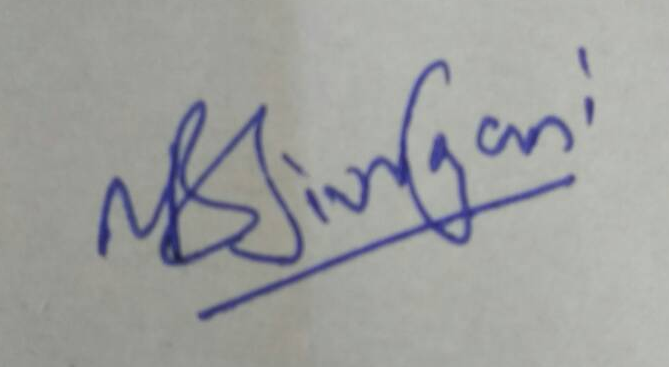
\includegraphics[width=3cm]{b}}



%\resheading{\textbf{STRENGTHS} }\\[\lsep]
%\begin{itemize}
%\item \noindent Positive Attitude, Social Interaction, Hardworking.
%\end{itemize}
%
%\resheading{\textbf{INTEREST AND HOBBIES} }\\[\lsep]
%\begin{itemize}
%\item \noindent Solving Puzzles.
%\item \noindent Playing Chess.
%
%\end{itemize}

\end{document}

